\chapter{Implementation}
\label{chapter6}

\section{Development Environment}
The development of this project was done in various environments, as there was many different aspects to this project.

\subsection{Vive Hardware}
	For this project, the Vive Hardware was set up in a dedicated room (The Virtual Reality Lab in the School of Computing). This allowed development to be done on the HTC Vive without having to set up the sensors and calibrate the hardware everytime that development had to be done, which maximised the amount of development time that was available.\\

\begin{figure}[H]
	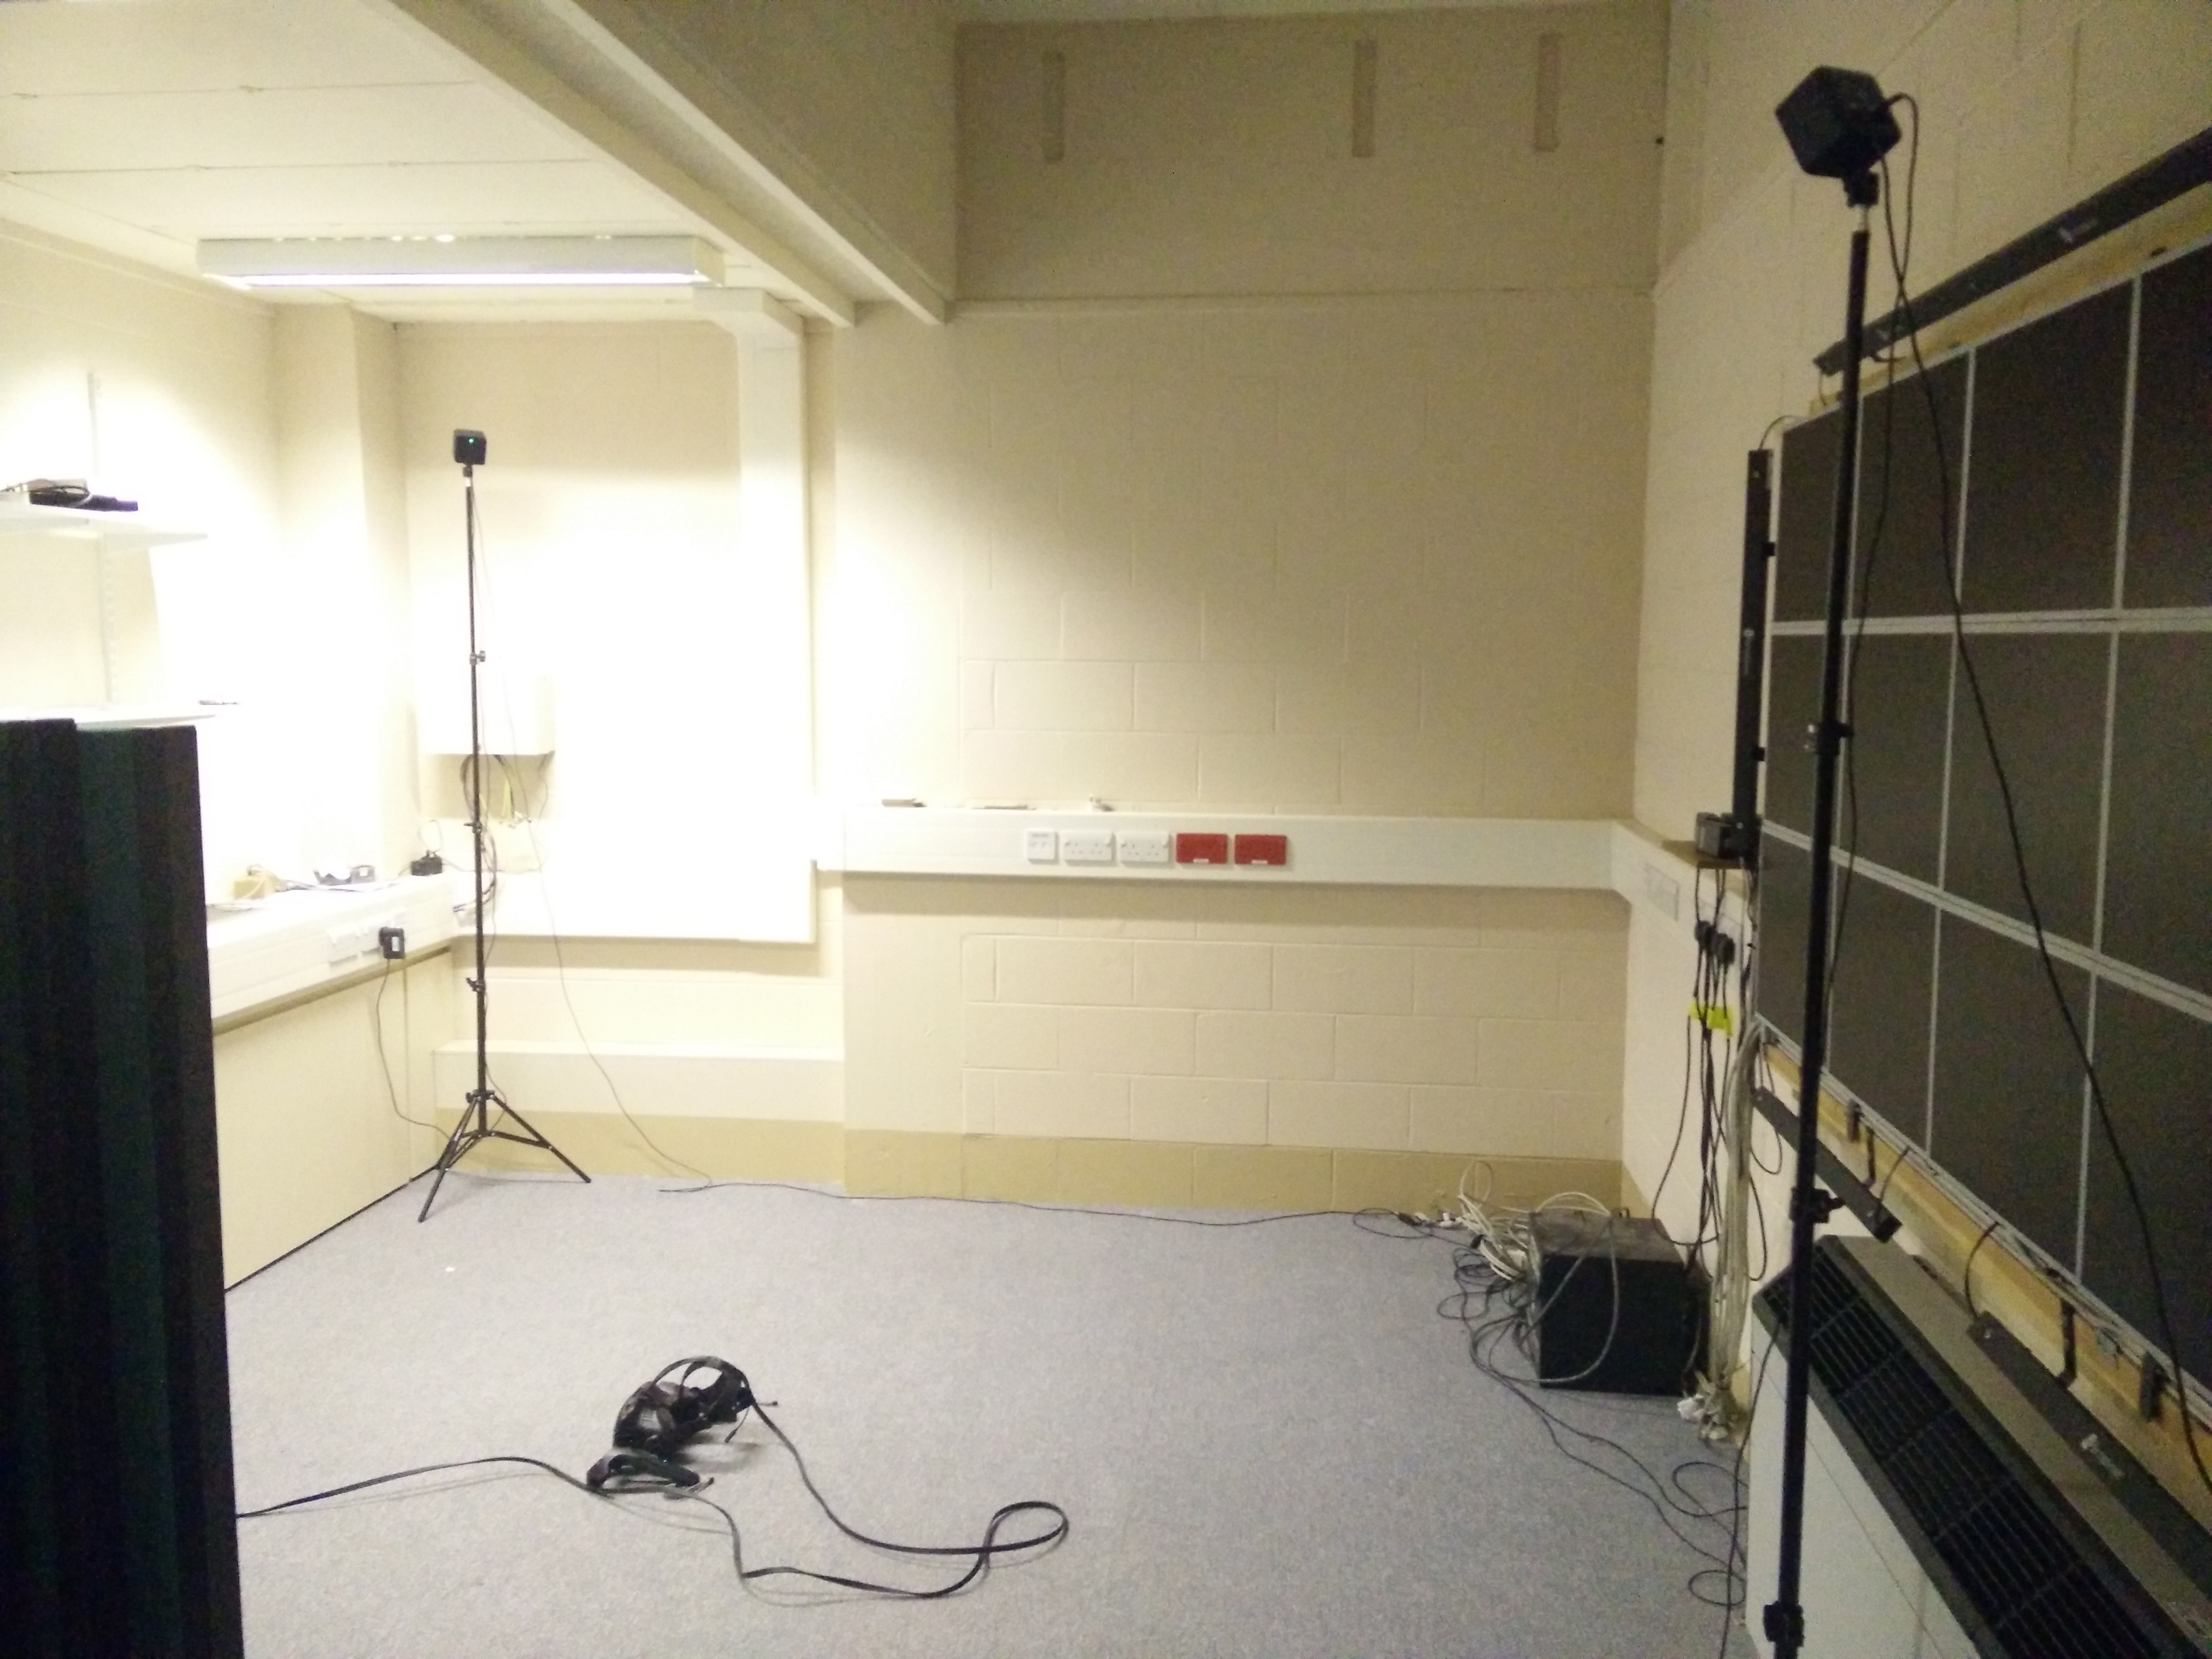
\includegraphics[width=\textwidth]{VRRoom}
	\centering
	\caption{Room used for testing the application}
	\label{fig:VRRoom}
\end{figure}

	This room was chosen as it was unused and met the space requirements for the HTC Vive.

\subsection{Game Engine}
\lipsum[1-1] \cite{parikh1980adaptive}

\subsection{Visual Studio}

\subsection{Windows}

\subsection{Out of Engine Development}
\lipsum[1-1] \cite{parikh1980adaptive}

\section{Random Generation of Graphs, Rivers and Terrain}

%Divide into sub sections as big topic
\subsection{Graph Generation Original Method}
\subsubsection{Point Insertion}
	The original idea to do graph generation was to start with a square, using each corner as a node. These nodes would then be connected as shown in \ref{fig:triangulation1}.\\

\begin{figure}[H]
	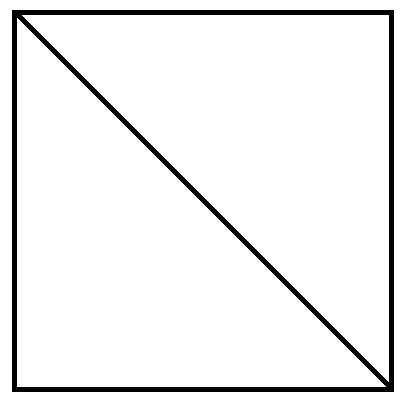
\includegraphics[width=10cm]{triangulation1}
	\centering
	\caption{Original Connections}
	\label{fig:triangulation1}
\end{figure}

	Points would then be inserted into this square, using a random x and y value.  The triangle that this node is in would then be found using the cross product. This was done by checking the cross product of the point and the triangle, for each triangle that is in the graph. The point would then be connected to the corners of this triangle.\\

\begin{figure}[H]
	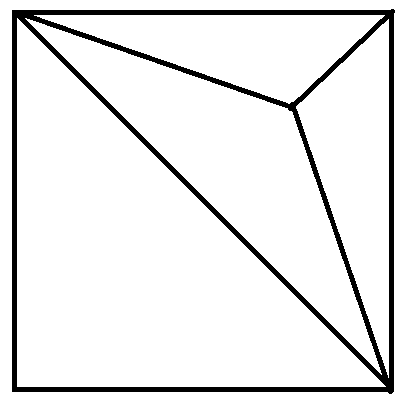
\includegraphics[width=10cm]{triangulation2}
	\centering
	\caption{Example of running the point insertion algorithm for one iteration.}
	\label{fig:triangulation2}
\end{figure}

\begin{figure}[H]
	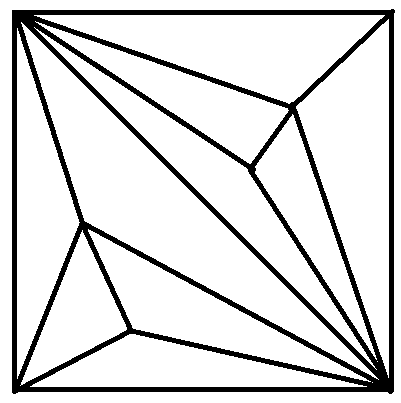
\includegraphics[width=10cm]{triangulation3}
	\centering
	\caption{Example of running the point insertion algorithm for four iterations}
	\label{fig:triangulation3}
\end{figure}

	This approach guaranteed a connected graph to begin with. This approach did not work however as if a node on the bottom-left side of the graph needed to be connected to a node on the top-right side of the graph, the the connection would have to be made through either the top-left node or the bottom-right node, as there was no other way to pass through to the other side of the graph. The approach was then modified slightly to start with an extra node node in the middle of the square, allowing another way to pass through the other side of the graph, this is seen in \ref{fig:triangulation4}.

\begin{figure}[H]
	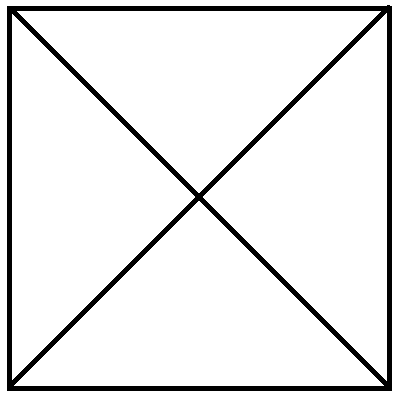
\includegraphics[width=10cm]{triangulation4}
	\centering
	\caption{Image showing the second method's starting connections}
	\label{fig:triangulation4}
\end{figure}
	
	This approach also did not work, as the addition of the extra node did not provide enough of relief for the connections between the two sides of the graph, and the connections would occasionally still go through the top-left or bottom-right node.
The next approach was adding seveeral nodes along the diagonal and connecting them to the corners, similarly to how the middle node was added. The third approach can be seen in \ref{fig:triangulation5}.

\begin{figure}[H]
	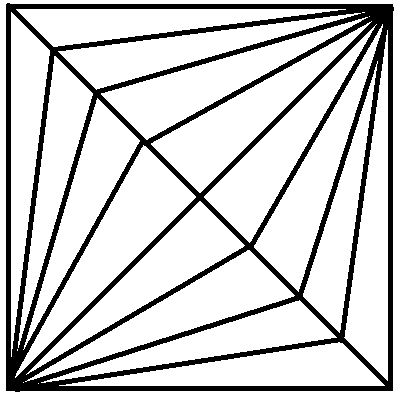
\includegraphics[width=10cm]{triangulation5}
	\centering
	\caption{Image showing the third method's starting connections}
	\label{fig:triangulation5}
\end{figure}

\subsubsection{Connections and Weight Matrix}
	The connections were found by looping through the array that stored the triangles and finding the edges of the triangles. These edges were stored in a connection matrix, to be used when making the weight matrix.\\
	The weight matrix was made using manhattan distance between the two connected points as the heuristic. The manhattan distance is the x distance between the two points plus the distance in the y direction. The manhattan distance was calculated using the following formula:\\

$$Manhattan = (point1.x - point2.x) + (point1.y - point2.y)$$
	
	The manhattan distance then has to be checked to see whether it is positive or not. If it is positive the result is put in element of the matrix representing the first point to the second point, if the result is negative the result is instead placed in the element representing the second point to the first point. This is repeated for each connection in the connection matrix produced before.

\subsubsection{Generating Rivers}
	The river generation starts off with picking the start and end nodes for the rivers, this is done by randomly selecting a set amount of nodes, determined by a variable set in code. 

\subsection{Terrain Generation}

\section{User Interactive Reverse Towers Of Hanoi}
The logic for the reverse Towers of Hanoi was implemented by using collision boxes on the rod actor to act as trigger when Towers of Hanoi discs are placed and removed. This method and actor was used as the basis and control for the Towers of Hanoi logic. To differentiate between the discs, three different actors were created for each size of the Towers of Hanoi discs: small, medium and large. 
\newline
\par
A collision box covers the whole rod with a size that is bigger thane the size of the hole in each disc is set to BlockAll so a disc cannot be placed through the rod. When an actor comes in contact with the collision box, this triggers the rod actor's OnHit collision event. Within this event, it identifies the size of the actor through the name of the actor's class and does a check with the array of discs in which that specific rod currently contains. This simple check will only allow discs which are larger to be placed on top of smaller discs and also makes sure that the array doesn't add disc actors that are already in the array. When the check is passed, the collision box's collision profile name is set to OverlapAll to allow the disc that triggered the event to be placed in that rod otherwise it sets it back to BlockAll. Furthermore, it adds an upward force to the disc to show that the action the player is trying to complete is invalid. This force is only added when the player is not holding the disc to avoid issues when the player is holding the disc and are moving/looking around and accidentally touching a rod with the disc.
\newline
\par
A second collision box that is slightly larger than the first was used to handle the adding and removing of discs to the array which contains all the disc actors which the rod currently holds. When a disc overlaps this collision box it adds it to the array through the OnOverlapBegin event trigger then removes it from the array with the OnOverlapEnd event trigger. When a disc is added to the array, it sets all the discs below it to not allow the player to grab it. This is done to keep with the Towers of Hanoi logic of only the disc at the top of stack being movable.
\newline
\par
A bonus feature to help with placing the discs was implemented with the `snap to rod' feature. When a disc is allowed to be placed on the rod so the disc is larger than the disc below it, then as soon as the OnOverlapBegin collision event is triggered, the disc is teleported to the top of the rod with its rotation reset so it can slide down the rod. This is useful as it can sometimes be bothersome to the player to place the disc exactly so the rod can fit exactly through the hole of the disc. This feature is only in effect when the disc is not currently being held by the player to avoid the disc teleporting whilst the player is still holding the disc which causes the disc to still be attached to the player's hand even though the disc is not in range of the hand's grab sphere.

\section{River Graph Flow}
Graph flow logic was implemented by using information generated with the terrain such as the nodes, IDs of rivers and knowing which rivers are connected to which. An actor for each river is created with a mesh using the UProceduralMeshComponent and the vertices supplied in the rivers.txt file. Each river is given an ID with the first part of the 2 numbers of the ID as the node the river is connected to and the last two numbers as the other node the other end of the river is connected to. This means that a series of river connections have the last two numbers of a river ID identical to the first two numbers of the next river in the connection.
\newline
\par
The source of the river in the graph has a flow value hard coded and then iterates through its river connection changing the flow value of each river then when it reaches the final river it means that the river has reached a node where it splits in to two. This split has a rod for each river in order for the player to change the flow of each river. With rods with no discs, the flow value is just split simply in half between the two rivers which then follows the same procedure as before and changes the flow value of the rivers in its river connections.
\newline
\par
With the case of rods with discs in them, the flow is then affected depending on which discs are used. A small disc will reduce the flow value of the river by a \(\frac{1}{6}\), medium disc by \(\frac{1}{3}\) and a large disc by \(\frac{1}{2}\). This means using all three discs would reduce the flow to 0 so completely blocking it off. Adding or removing a disc from a rod would change the flow value for the river the rod is connected to which then changes the flow value of all the rivers that this river affects.
\newline
\par
In order for the player to easily distinguish a difference in the flow of a river when changing them with the discs, the opacity of the material used on the river will change depending on the flow value as a percentage of the original flow value at the source.

\section{Flow Dependant Flora}
\lipsum[1-1] \cite{parikh1980adaptive}